\begin{thm}{073}{\hosi 8}{学コン}
 $\mr{AB}=1$, $\mr{AC}=\sqrt{3}$, $\angle\mr{A}=90^\circ$ の$\triangle\mr{ABC}$の外接円をTとおく。端点除く辺$\mr{BC}$上にある点P, Qは、$\angle\mr{BAP}=\angle\mr{CAQ}=\theta$を満たす。線分AP, AQの延長とTの交点をそれぞれR, Sとし、$\dfrac{\triangle\mr{ACS}}{\triangle\mr{BPR}}$が最小になるときの最小値、及びBP, CQの長さを求めよ。
\end{thm}

\begin{figure}[H]
 \centering
 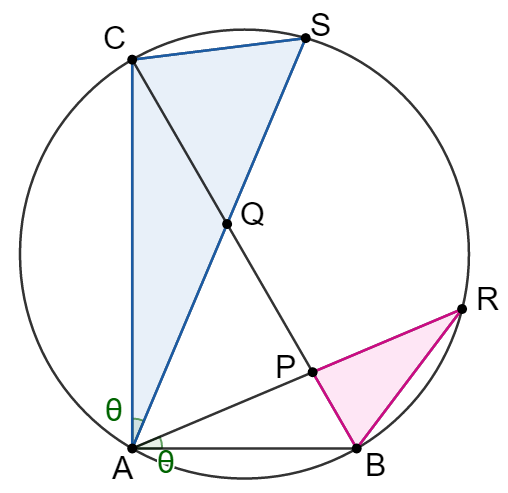
\includegraphics[width=0.5\linewidth]{../problems/Q_073/A_073.png}
\end{figure}
$\angle\mr{CAS}=\angle\mr{PAB}=\theta$, $\angle\mr{ASC}=\angle\mr{ABP}=60^\circ$なので、$\triangle\mr{ACS}\sim\triangle\mr{APB}$である。この相似比は$\mr{AC}:\mr{AP}$であるから、面積比は$3:\mr{AP}^2$。一方で、
\[ \triangle\mr{APB}:\triangle\mr{BPR} = \mr{AP}:\mr{RP} = \mr{AP}^2:\mr{AP}\cdot\mr{RP} \]
だから、$\triangle\mr{ACS}:\triangle\mr{BPR}=3:\mr{AP}\cdot\mr{RP}$。続いて方べきの定理によって、$\mr{AP}\cdot\mr{RP}=\mr{BP}\cdot\mr{CP}$となる。$\mr{BP}=x$とおくと、$\mr{CP}=\mr{BC}-\mr{BP}=2-x$なので、
\[ \mr{BP}\cdot\mr{CP}=x(2-x)=-(x-1)^2+1 \]
となる。したがって、
\[ \frac{\triangle\mr{ACS}}{\triangle\mr{BPR}}=\frac{3}{-(x-1)^2+1} \]
は$x=1$のときに最小となり、その値は$3$である。

このとき$\mr{BP}=x=1$である。また$\mr{AB}=\mr{BP}$と$\angle\mr{ABP}=60^\circ$であるから$\triangle\mr{APB}$は正三角形で、$\theta=60^\circ$。よって$\angle\mr{BAQ}=90^\circ-\theta=30^\circ$とあわせて、$\mr{BQ}=\dfrac{1}{2}$とわかる。したがって、$\mr{CQ}=\mr{BC}-\mr{BQ}=\dfrac{3}{2}$。